\section{Type Ia Supernova} \label{sec:sn_ia}

For many centuries, astronomers all over the globe would observe the emergence of a bright light in the sky thinking it was the birth of a new star in the Universe. 
In 1572, an astronomer by the name of Tycho Brahe developped an interest in such event and named the phenomenon \textit{nova stella}, latin for new star. 
His work inspired later astronomers suhc as Kepler and eventually lead to the Copernicean revolution.\\

It wasn't until 1934 when Fritz Zwicky and Walter Baade when the term supernova (from the latin "super" and "novae" meaning new bright stars) was coined to describe the 
brightest novae observed. The supernova classifies phenomena related to the end of a star's life cycle when they go through explosions. This process is temproary therefore 
taking part in the class of \textbf{transients}. Their fluxes are initially weak and then increases over time to a point where it becomes detectable from 
the Earth, then it diminishes slowly till it disapears.\\

In the next sections we will be explaining the different classifications of supernovae as well as our understanding behind their explosion mechanisms. A particular focus 
will be on a specific class of supernovae called "type Ia" and why they are heavily studied by cosmologists. \\

\subsection{Classification}

Two main categories of supernovae exists: type I and tpye II each with their own subcategories of supernovae. These main categories were discovered by Rudolph Minkowskia and 
Walter Baade in 1941 when studying the spectral features of 14 supernovae. Type I supernovae's absorption spectra is characterized by having no Hydrogen, contrary to type II. 
Type I supernova are then divided in two three classes (\cite{Wheeler_1985, Elias_1985}, \cite{Wheeler_1990}):
\begin{itemize}
    \item \textbf{Ia}: contains Silicon line at $615.0$ nm
    \item \textbf{Ib}: does not contain Silicon and contains Helium line at $587.6$ nm 
    \item \textbf{Ic}: does not contain Silicon or Helium lines
\end{itemize}

\noindent Type II supernova are divided in following way (\cite{Hillier_2019}):
\begin{itemize}
    \item \textbf{IIn}: contains narrow absoption lines
    \item \textbf{IIb}: contains Helium like Ib 
    \item \textbf{IIP}: Hydrogen dominates the spectra and its integrated flux becomes constant
    \item \textbf{IIL}: Hydrogen dominates the spectra and its integrated flux decreases in time
\end{itemize}

\noindent The classification of supernovae can be summarized in Figure \ref{fig:sn_classification}.

\begin{figure}[ht]
    \centering
    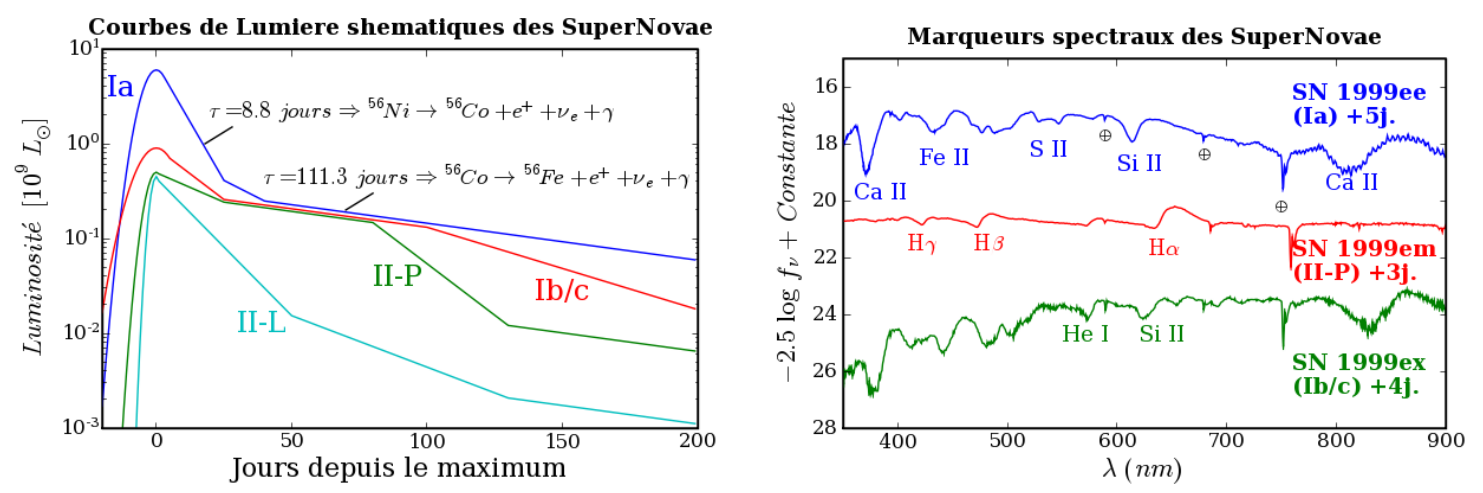
\includegraphics[width=1.0\textwidth]{MainLayout/Second_chapter/figures/sn_class_lc_spec.png}
    \caption{Photometric and spectroscopic curves for different classes taken from \cite{Baumont_2007}. 
            The left are the schematics for the integrated fluxes (lightcurves) for SN Ia (blue), SN Ib or Ic (red), SN IIP (green) and SN IIL(cyan). 
            On the right we have the spectra of three supernovae observed in 1999, SN Ia (blue), SN IIP (red) and SN Ic (green).}
    \label{fig:sn_classification_spec}
\end{figure}

\begin{figure}[ht]
    \centering
    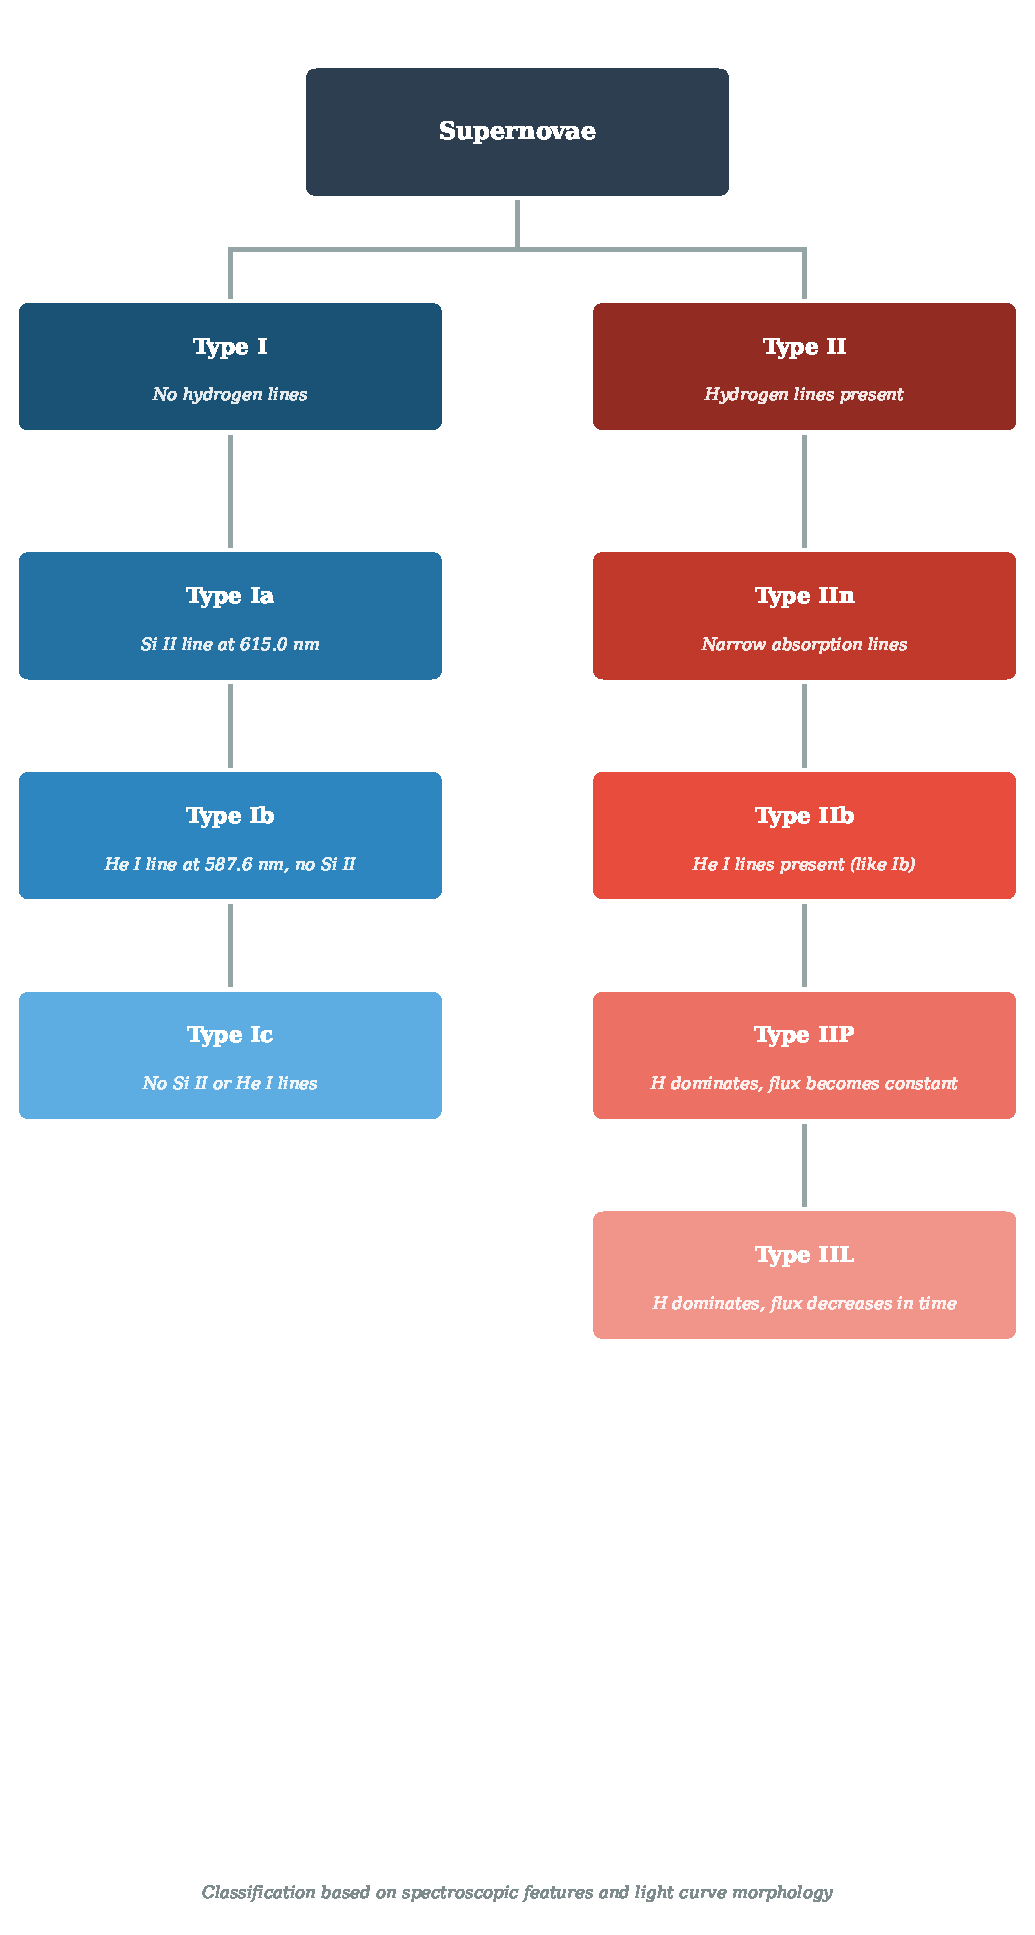
\includegraphics[width=0.7\textwidth, trim=0cm 9cm 0cm 0cm, clip]{MainLayout/Second_chapter/figures/sn_classification_vertical.pdf}
    \caption{Classification of supernovae. The left column are type I (blue) and the right column are tpye II (red).}
    \label{fig:sn_classification}
\end{figure}

\subsection{Explosion mechanisms}

Different explosion mechanisms and progenitors exist for the different classes of supernovae. We will be separating them into two cases: core-collapse and thermonuclear.\\

\noindent \textbf{\underline{Core collapse}} \\

This explosion concerns supernovae of types Ib, Ic and all types II. The occurence of this explosion happens at the end of the life cycle of a star after it has 
completed the fusion of its light elements. The star then does generate enough energy to compensate for the gravitational pull and then collapes on itself. The material 
of the star collapses until it reaches scales at which it is stopped by the strong nuclear interaction, which defines the limiting distance between atoms. This causes a collision 
between the different layers of the star creating a shock wave  that propulses the star material and ignites the supernova explosion. If the star has a mass inferior to 
$\sim 3.3M_{\odot }$ (Oppenheimer-Volkoff limit \cite{Oppenheimer_1939}), where $\bigodot$ denotes the Solar mass, the star will become neutron star. Larger mass stars turn to black holes.\\



\noindent \textbf{\underline{Thermonuclear}} \\

Thermonuclear explosions concern tpye Ia supernovae. This occurs in white dwarf stars comprised primarily of Oxygen and Carbon when their masses approach the Chandrasekhar limit 
of $\sim 1.44M_{\odot }$ (\cite{Chandrasekhar_1931}). White dwarf stars form from the remains of low mass stars (typically under $8M_{\odot}$) and are dense degenerated systems. 
This term comes from the fact that the density of a white dwarf is limited by electron degeneracy pressure that comes from the Pauli exclusion principle which states that 
two electron within the same energy levels cannot share the same quantum state. Accreting more mass from external sources induces Carbon and Oxygen fusion which increases 
the temperature of the white dwarf stars. If the accretion keeps on happening, the fusion of Carbon and Oxygen becomes a chain reaction at a constant pressure causing a 
thermonuclear explosion (\cite{Ropke_2004}). The explosion ends up releasing around $10^{51}$J of energy, mainly kinetic energy. Only a fraction of that is turned into luminous energy 
of $10^{44}$J (\cite{Khokhlov_1993}) meaning tpye Ia supernovae have a luminosity at the same order of magnitude of its host galaxy. \\

Observations such as SN2011fe have demonstrated that type Ia supernovae are originated from compact and dense stars, which are white dwarfs. It also important to note that 
tpye Ia supernova spectra are characterized by Silicium and Calcium absoption lines which are the product of the Carbon and Oxygen fusion. Due to the fact that 
type Ia supernovae occur in quasi-identical environments, we tend to observe similar luminosities between them. Finally, they are observed in environments with older stars 
which is justified due to the fact that white dwarfs happen at the final stages of a star. \\

White dwarf stars aren't very luminous to be observed at long distances. Usually they are detected a short while after their explosions. Therefore the progenitors of type Ia 
supernovae have never been observed. Multiple scenarios exist to explain the explosions. We will only be presenting the two main scenarios:
\begin{itemize}
    \item \textbf{Single degenerate} (\cite{Nomoto_1982}): This occurs when white dwarfs accrete mass from nearby more massive non-degenerate stars will low surface gravity, like red giants. 
Arguments against that scenario is that the accreted Helium and Hydrogen must all be transformed into Carbon and Oxygen with a fusion reaction, which would explain why they do not appear as absorption line 
in the spectrum of the supernova. The other is that the speed of the accretion can neither be too slow nor too fast or the explosion doesn't happen. Lastly, the companion stars 
weren't observed near the explosion area (\cite{Li_2011}).
    \item \textbf{Double degenerate} (\cite{Iben_1984}): This occurs when a white dwarf star accretes its mass from a nearby less massive white dwarf star in close orbit. This scenario does explain
the absence of Helium and Hydrogen absoption lines and the observation of superluminous supernovae (like \cite{Howell_2006}). It also allows for the case of a double detonation which when it happens 
for two white dwarfs who's masses are inferor to the Chandrasekhar mass can explain the existence of subluminous supernovae (\cite{Tanikawa_2019}).
\end{itemize}


\subsection{Explosion rate}

The explosion rate of type Ia supernovae is the measurement of the number of explosion at a certain redshift in year. 
It can be divided into two categories: low redshift up to $z \sim 0.3$ and hight redshift. At low redshift the explosion is nearly constant 
and barely evolves. Low redshift samples such as ZTF allow us to measure that rate. A study done by \cite{Perley_2020} on the ZTF sample, assuming an isotropic distribution, 
have measured a rate of
\begin{equation}
    R_{ZTF} = (2.35 \pm 0.24) \times 10^{4} \text{Gpc}^{-3}.\text{yr}^{-1}
\end{equation}
Where each supernova was weighted by the volume it probes with a varying limiting absolute magnitude. 
However, a recent paper by \cite{Lordet_2026} showed that the rate of supernova is explosion might be more complex than anticipated and is much more dependent on its environment. 
Figure \ref{fig:sn_rate_antoine} highlights that the assumption that the rate is homogenous at low redshift isn't sufficient to describe supernova as we observe an excess 
at $z \sim 0.035$ while Figure \ref{fig:sn_vs_delta_antoine} shows that the excess of supernova at that redshift seems to be located arond extremely dense regions. \\

At high redshift the rate becomes very dependent on the redshift. Its behaviour can be described by a power law with respect to $(1+z)$. Estimates by combining 
a multitude of probes in \cite{Frohmaier_2019} have shown that the rate can be described as:
\begin{equation}
    R(z) = (2.27 \pm 0.19)\times 10^{4} \times (1+z)^{(1.70\pm 0.21)} \text{Gpc}^{-3}.\text{yr}^{-1}
\end{equation}

\begin{figure}[ht]
    \centering
    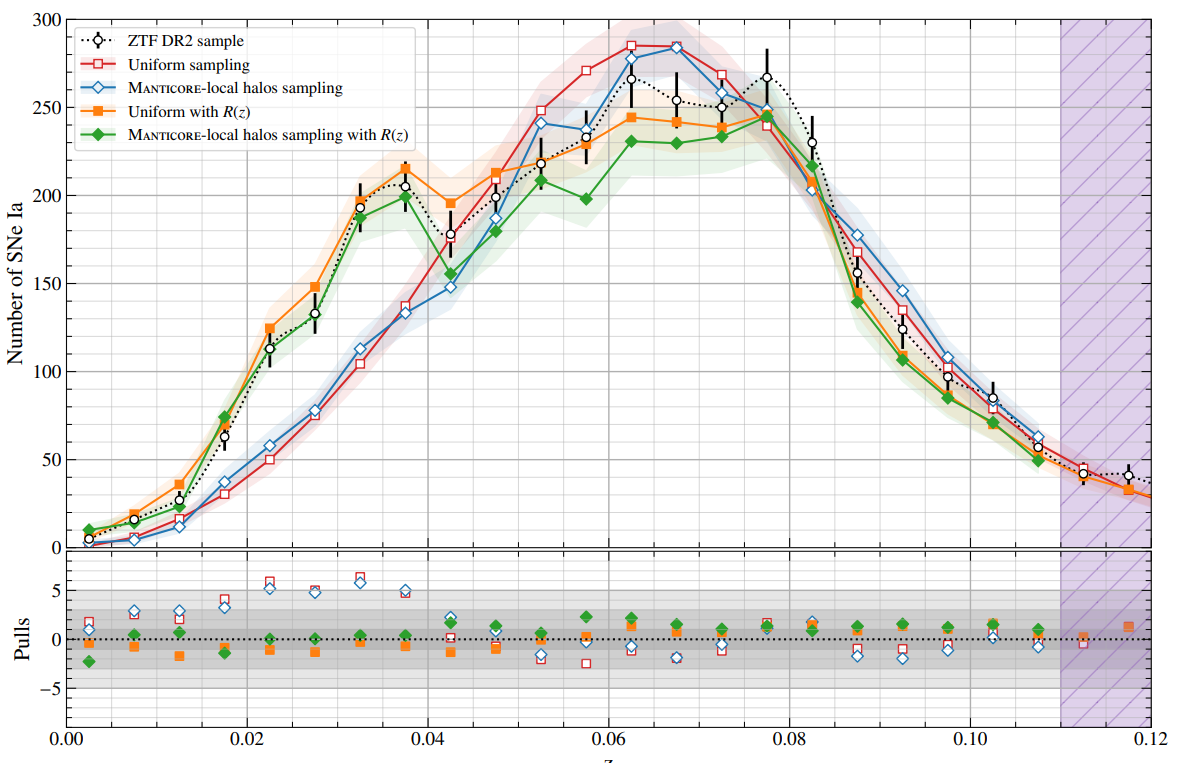
\includegraphics[width=0.8\textwidth]{MainLayout/Second_chapter/figures/sn_rate.png}
    \caption{Distribution of simulated supernova observed as a function of redshift $z$ vs the ZTF DR2 sample of obsereved supernovae (circle with black uncertainty). The different simulations are done using different priors on their positions. Red assumes a uniform sampling like \cite{Perley_2020}. Blue uses a uniform sampling weighted by halo masses from Manticore-local. Oragne assumes a redshift dependent rate. Green assumes a redshift dependent rate and weights by the halo masses.}
    \label{fig:sn_rate_antoine}
\end{figure}

\begin{figure}[ht]
    \centering
    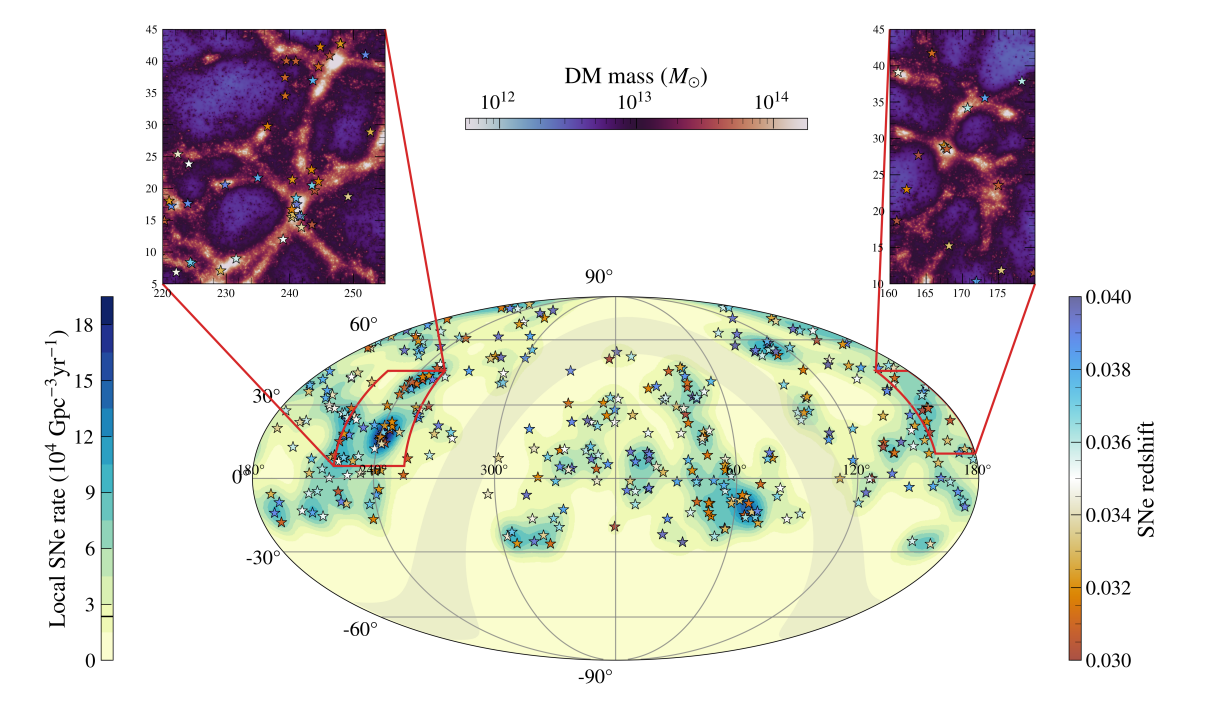
\includegraphics[width=1.0\textwidth]{MainLayout/Second_chapter/figures/sn_vs_delta.png}
    \caption{Distribution of supernova obsereved vs the dark matter distribution posterior from Manticore-local as well as the local supernova rate. Top left corner we have a zoom in on the Hercules supercluster. Top right corner we have a zoom in on the Leo supercluster.}
    \label{fig:sn_vs_delta_antoine}
\end{figure}

\subsection{Observations}

\noindent \textbf{\underline{Spectroscopic}} \\

Type Ia supernova spectra have a distinct spectra. Most of the light emitted from a type Ia is in the visible wavelengths with some parts of their spectra in the infrared and ultraviolet. 
During the initial phases of the explosion the external layers of the explosion are opaque. Near the maximum emission of light, we expect to see 
absoption lines of Silicium and Calcium caused by the fusion of Carbon and Oxygen. The days that follow, the opacity decreases and we start to see absoption lines 
from Nickel and Cobalt. Finally, in the following weeks the Nickel and Cobalt will disintegrate into Iron for which we see the absoption lines. \\

\begin{figure}[ht]
    \centering
    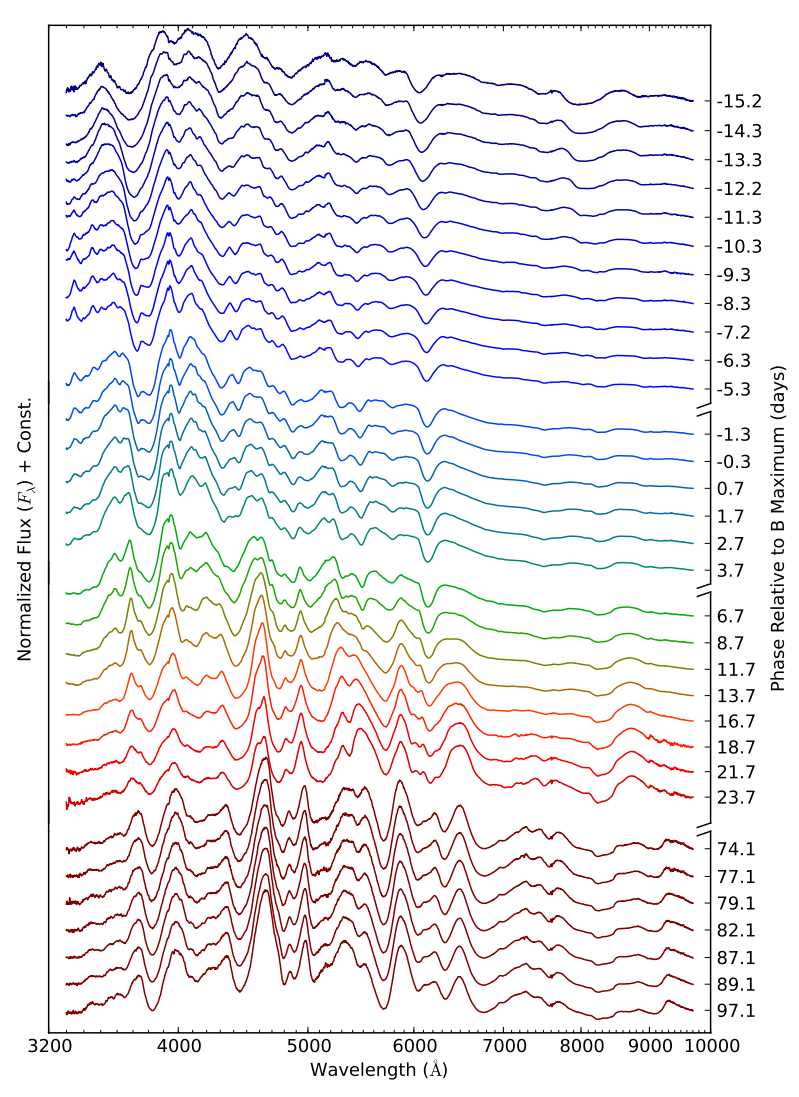
\includegraphics[width=0.7\textwidth]{MainLayout/Second_chapter/figures/sn2011fe_spectra_.png}
    \caption{Spectral series of SN 2011fe supernova taken by with the SNIFS instrument (\cite{Pereira_2013}). The spectra were captured betwenen -15 days to 50 days after the maximum emission data. They are ordered from top to bottom, or blue to red. The magnitude shown are relative to the maximum magnitude.}
    \label{fig:sn_spectra_2011fe}
\end{figure}

\noindent \textbf{\underline{Photometric}} \\

When describing the photometric evolution of type Ia supernovae, we are describing the integrated flux in a observation band or filter that covers a specific wavelength. Generally, 
we use the standard filters U, B, V, R and I (also known as the Bessel filters \cite{Bessell_1990}) that cover the ultraviolet, visible and near-infrared range.
We observe in all bands an increase the lightcurve that lasts approximately 20 days with an absolute magnitude in the B band of $-19.5$mag that occurs following the 
disintegration of Nickel. After that, the visible and ultraviolet bands measure an exponential decrease due to the disintegration into Iron. In the infrared bands, we observe 
a second peak somwhere between 20 to 25 days after the first peak. \\

\begin{figure}[ht]
    \centering
    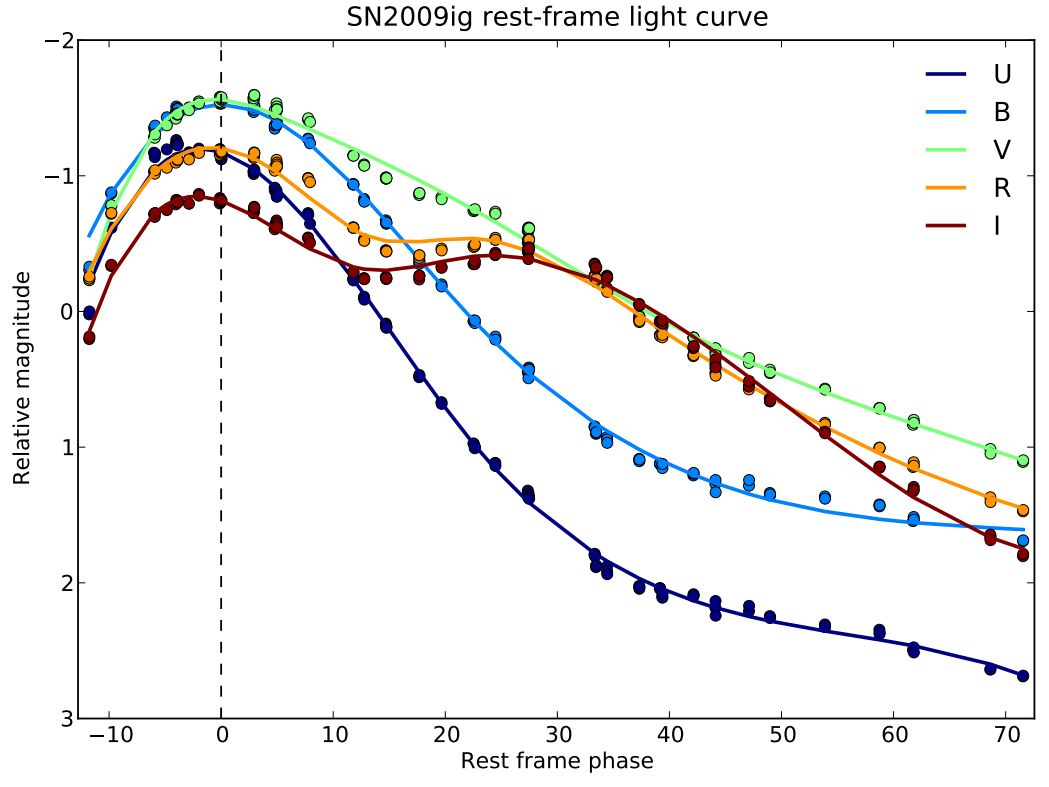
\includegraphics[width=0.7\textwidth]{MainLayout/Second_chapter/figures/sn2009ig_lightcurve.png}
    \caption{Synthetic lightcurves of the SN 2009ig supernova in the UBVRI bands made for the SNfactory collaboration taken from \cite{Chotard_2011}.}
    \label{fig:sn_lc_2009ig}
\end{figure}

